\section{\tool{} Leakage Definition}
In the section, we discuss how \tool{} quantifies the amount of
leaked information. \tool{} is a dynamic-based approach to 
quantify the information leakage. We will first introduce 
the limitation of existing quantification metrics. After
that, we introduce the abstract and notation for the paper 
and propose our method.

\subsection{Problem Setting}
Existing static-based side-channel quantification works~\cite{182946,Wichelmann:2018:MFF:3274694.3274741 } define information leakage
using max entropy or Shannon entropy. These definitions provide a strong security guarantee
when trying to prove a program is secure enough if zero bit of information is leaked 
reported by their approaches. However, it is useless if the tool report the program leaks
some information. Moreover, those metrics does not apply to static method.


\begin{figure}[h!]
    \centering
\begin{lstlisting}[xleftmargin=.03\textwidth,xrightmargin=.01\textwidth]
uint8_t password = input();
if(password == 0x1b){
    pass();     //branch 1
}else{
    fail();     //branch 2
}
\end{lstlisting}
\caption{A dummy password checker}
\label{figure:password checker}
\end{figure}

We consider the above dummy password checker~\ref{figure:password checker}.
The program will take a 8 bit number as the input and check if the input is the
correct password. 
If an attacker knows the
code executes branch $\{{1\}}$ by side-channel attacks, he can infer the password equals to 0x1b,
in which case the attacker can fully retrieve the password.
Therefore, the total information leakage should be 8 bits, which equals to the size
of the sensitive input. 

However, previous static-based approach can not precisely reflect the sensitivity of the leakage.
According to the definition of Shannon entropy, the leakage will be $\frac{1}{256}*\log_{2}\frac{1}{256} + 
\frac{255}{256} *\log_{2}\frac{255}{256}= 0.24$ bits. Because the program has two branches, tools
based on max-entropy will report the code has $log_2{2} = 1$ bit leakage.

Both approaches fail to tell how 
much information is leaked during the execution precisely.

The problem with the existing methods is that they are static-based and the 
input values are neglected by the previous definition. 
They assume the attacker runs the program multiple times with many different sensitive 
information as the input. Both Shannon entropy and max entropy give an ``average" 
estimate of the information leakage. However, it is not the typical scenario for an adversary to 
launch a side-channel attack. When a side-channel attack happens, the adversary wants 
to retrieve the sensitive information, in which case the sensitive information is fixed (e.g. AES keys). 
The adversary will run the attack over and over again and guess the value bit by bit. Like the 
previous example, the existing static method does not work well in those situations.

\begin{figure}
  \centering
   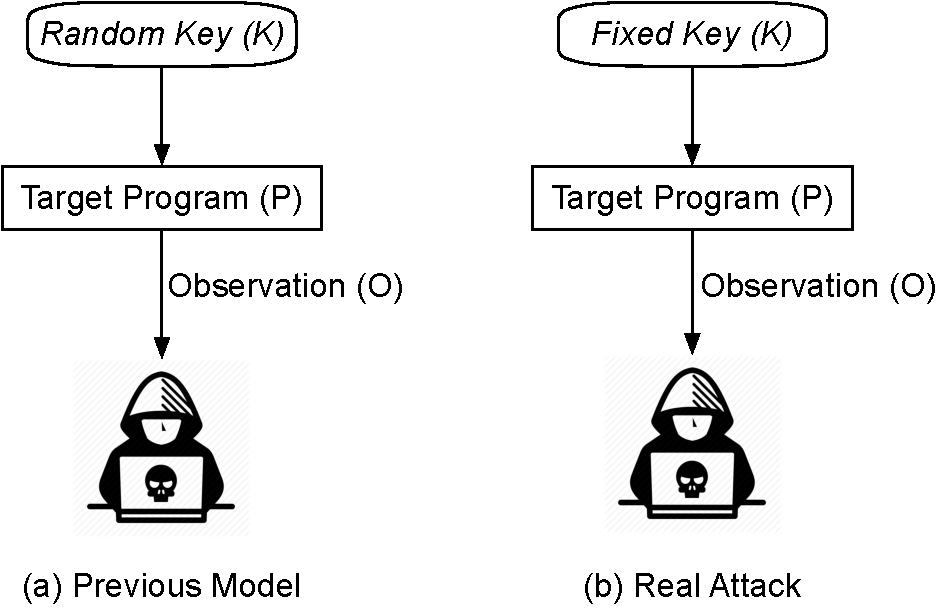
\includegraphics[width=.9\columnwidth]{./figures/RA.pdf}
   \caption{The gap between the real attack and previous model}
\end{figure}


\subsection{Notations}
In the section, we give the necessary definitions and notations for dealing 
with programs and side-channels.
We assume the program ($P$) has $K$ as the sensitive input. 
$K$ should be a finite set of keys. The program also takes known messages $M$ as the input. The model applies to most of the most cryptosystems. For example,
during the AES encryption, $P$ are the encryption function. $K$ is AES key and
$M$ is the message to be encrypted. During the execution, an adversary may have some observations ($O$) from the program. Examples of those observations
include timing, CPU usages, and Electromagnetic signals (EM). For the paper, we
consider the secret-dependent control-flows and secret-dependent memory accesses
as the observations.

With the above definitions, we have the following functions:
\begin{displaymath}
    P(K, M) \rightarrow	O
\end{displaymath}

An adversary does not have access to $K$, but he should know $P$, $M$, and $O$. 
For one execution of a deterministic program, once $k \in K$ and $m \in M$ are fixed, the 
observation ($o \in O$) is also determined. As an attacker, he knows $P$, $o$, 
and $m$ and wants to infer value of $k$. We use $\hat{K}$ to denote the set of
$k$ that satisfies the below function:

\begin{displaymath}
    P(\hat{K}, m) \rightarrow	o
\end{displaymath}
The problem of quantifying the amount of leaked information can be transferred into the
following question: 

How much uncertainty of $K$ can be reduced if an attacker knows $P$, $m$, and $o$?  

\subsection{Theoretical Analysis}
Suppose a program with some
sensitive input $K$, an adversary has some observations ($O$) by side channels.  
 %In this work, the observations are referred as the secret-dependent control-flows and
 %secret-dependent data-access patterns. 
  The conditional entropy $H(K|O)$ is
\begin{displaymath}
    H(K|O) = - \sum_{o_j {\in} O} {P(o_j) \sum_{k_i {\in} K}{P(k_i|o_j)\log_2P(k_i|o_j)}}
\end{displaymath}
Intuitively, the conditional information marks the uncertainty about $K$ after the adversary
has gained some observations ($O$). 

Some previous work uses the mutual information $I(K; O)$ to quantify the leakage which is defined 
as follows:
\begin{displaymath}
    \mathit{Leakage} = I(K;O) = \sum_{k_i {\in} K}{\sum_{o_j {\in} O}{P(k_i, o_j)\log_2\frac{P(k_i, o_j)}{P(k_i)P(o_j)}}}
\end{displaymath}
where $P(k_i, o_i)$ is the joint discrete distribution of $K$ and $O$.
Alternatively, the mutual information can also be computed with the following equation:
\begin{displaymath}
    \mathit{Leakage} = I(K;O) = H(K) - H(K|O) = H(O) - H(O|K)
\end{displaymath}

For a deterministic program, once the input $K$ is fixed, the program will have the same
control-flow transfers and data-access patterns. As a result, $P(k_i, o_j)$ will always
equals to 1 or 0. So the conditional entropy $H(O|K)$ will equal to zero. So the leakage defined
by the mutual information can be simplified into:
\begin{displaymath}
\label{mutual:information}
    \mathit{Leakage} = I(K;O) = H(O)
\end{displaymath}
In other words, once we know the distribution of those memory-access patterns. We can 
calculate how much information is actually leaked.

In the project, we hope to give a very precise definition of information leakages. 
Suppose an attacker run the target program multiple times with one fixed input, we
want to know how much information he can infer by observing the memory access patterns.
We come to the simple slogan ~\cite{10.1007/978-3-642-00596-1_21} %% where the information
%% leakage equals:
%% \textbf{Initial uncertainty - remaining uncertainty}
that
\begin{align*}
 & \mathit{Information\ leakage} = \\
 & ~~~~~~ \mathit{Initial}\ \mathit{uncertainty} - \mathit{Remaining\ uncertainty}. 
\end{align*}


If an adversary has zero knowledge about the input before the attack. The initial uncertainty
equals to the size the input. As for the remaining uncertainty, we come to the original definition
of the information content.
We quantify the information leakage with the following definition. 

\newtheorem{mydef}{Definition}

\begin{mydef}
\label{def}
Given a program $P$ with the input set $K$, 
an adversary has the observation $o$ when the input $k{\in}K$. 
We denote it as
    $$P(k) = o.$$
The leakage $L_{P(k)=o}$ based on the oberservation is
    $$L_{P(k)=o} = \log_2{|K|} - \log_2{|K^o|}$$
    where
    $$K^o = \{k | k \in K \ \text{and} \ P(k) = o \}$$
\end{mydef}

With the new definition, if the attacker observes that the code~\ref{code::entropy} runs the branch 1, 
then the $K^{o^{1}} = \{128\}$. Therefore, the information leakage $L_{P(k)=o^{1}} = \log_2{256} - \log_2{1} = 8$
bits, which means the key is totally leaked. If the attacker observes the code runs other
branches, the leaked information is shown in the following table.

\begin{table}[h]
    \centering
    \resizebox{.7\columnwidth}{!}{
    \begin{tabular}{|c|c|c|c|c|}
    \hline
    Branch & 1 & 2  & 3  & 4   \\ \hline
    $K^o$   & 1 & 64 & 64 & 127 \\ \hline
    $L_{P(k)=o}$(bits)   & 8 & 2  & 2  & 1   \\ \hline
    \end{tabular}
    }
    \caption{The leaked information by the definition~\ref{def}}
\end{table}

With the same definition~\ref{def}, if the attacker observes that the code run branch 2, the information
leakage will be 2 bits. The conclusion is consistent with the intuition. Because if the branch 2 was
executed, we can know the key is less than 64. So we know the most and the second significant digits of 
the value key equals to $128$.

